%
% LaTeX report template 
%

% This is a comment: in LaTeX everything that in a line comes
% after a "%" symbol is treated as comment

\documentclass[11pt, a4paper]{article}
\usepackage{graphicx}
\usepackage{amsmath}
\usepackage{listings}


\title{Assignment No 6} % Title

\author{Prasanna Bartakke EE19B106} % Author name

\date{\today} % Date for the report
\begin{document}		
		
\maketitle % Insert the title, author and date
\section{Introduction}
%Create new section;it is autonumbered
In this assignment a 1D model of a tube light is simulated. A uniform electric field is present, that accelerates electrons. Electrons are emitted by the cathode with zero energy, and accelerate in this field. When they get beyond a threshold energy $E_0$, they can drive atoms to excited states. The relaxation of these atoms results in light emission. 
\section{Taking input from user or using predifined parameters}
\begin{verbatim}	
if len(sys.argv)==6:
    n=sys.argv[0]       # spatial grid size.
    M=sys.argv[1]       # number of electrons injected per turn.
    nk=sys.argv[2]      # number of turns to simulate.
    u0=sys.argv[3]      # threshold velocity.
    p=sys.argv[4]       # probability that ionization will occur
    Msig=sys.argv[5]    # deviation of elctrons injected per turn
    param = [n,M,nk,u0,p,Msig]
else:
    param = [100,5,500,5,0.25,2] 
\end{verbatim}
\section{The Simulation Loop}
\begin{verbatim}
def simulate(params):
    n = params[0]
    M = params[1]
    nk = params[2]
    u0 = params[3]
    p = params[4]
    Msig = params[5]
    xx = np.zeros((n*M))  # electron position
    u = np.zeros((n*M))   # electron velocity
    dx = np.zeros((n*M))  # displacement in current turn

    I = []
    V = []
    X = []
    
    for i in range(1, nk):
        ii = where(xx>0)                #indices of positions greater 
                                        #than zero
        dx[ii] = u[ii] + 0.5            #displacement
        xx[ii] += dx[ii]                #update position
        u[ii] += 1                      #update velocity

        overshoot = where(xx[ii]>n)     #contains the indices whose disp, 
                                        #vel, pos have to set to 0
        xx[ii[0][overshoot]] = 0
        u[ii[0][overshoot]] = 0
        dx[ii[0][overshoot]] = 0


        kk = where(u>=u0)               #v greater than threshold
        ll = where(rand(len(kk[0])) <= p)
        kl=kk[0][ll]                    #contains the indices of energetic 
                                        #electrons that suffer collision
        u[kl]=0                         #velocity becomes 0 after collision
        
        rho = rand(len(kl)) 
        xx[kl] = xx[kl]-dx[kl]*rho      #actual value of x where it collides

        I.extend(xx[kl].tolist())

        m = int(rand()*Msig + M)        #number of new electrons to be added
        vacant = where(xx==0)           #empty spaces where electrons 
                                        #can be injected
        nv=(min(n*M-len(vacant),m)) 
        xx[vacant[:nv]]=1               #inject the new electrons
        u[vacant[0][:nv]]=0             #velocity zero
        dx[vacant[0][:nv]]=0            #displacement zero
        X.extend(xx.tolist())
        V.extend(u.tolist())
    return X,V,I
\end{verbatim}
\section{The different plots}
{\bf plot\_intensity} to plot the intensity vs x.
 
   \begin{figure}[!tbh]
   	\centering
   	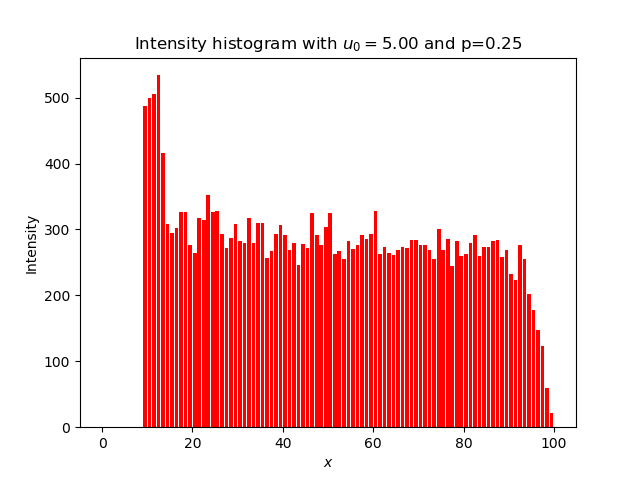
\includegraphics[scale=0.5]{fig0.png}  % Mention the image name within the curly braces. Image should be in the same folder as the tex file. 

   	\label{fig:sample}
   \end{figure} 


{\bf plot\_no\_of\_elec} to plot the number of electrons vs x.
 
   \begin{figure}[!tbh]
   	\centering
   	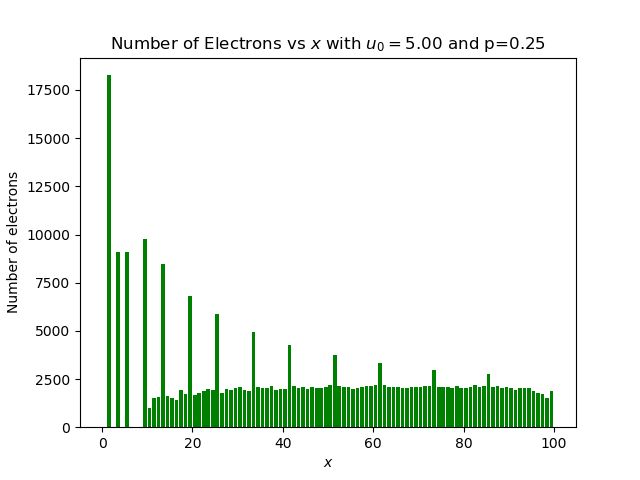
\includegraphics[scale=0.5]{fig1.png}  % Mention the image name within the curly braces. Image should be in the same folder as the tex file. 

   	\label{fig:sample}
   \end{figure} 
   
{\bf plot\_phase\_space} to plot the phase space of electrons.
 
   \begin{figure}[!tbh]
   	\centering
   	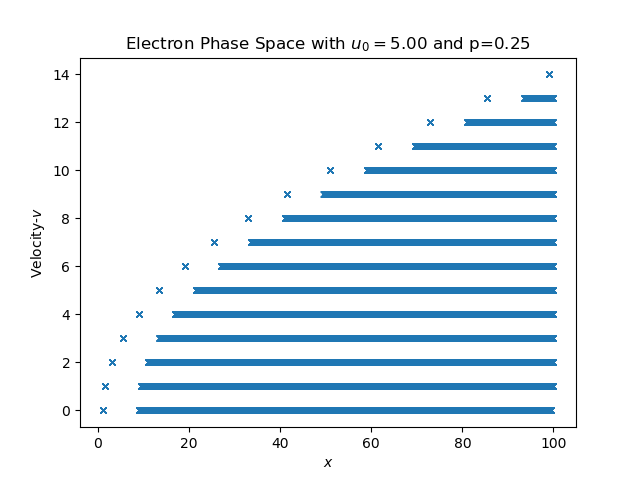
\includegraphics[scale=0.5]{fig2.png}  % Mention the image name within the curly braces. Image should be in the same folder as the tex file. 

   	\label{fig:sample}
   \end{figure} 
  
  {\bf plot\_intensity\_map} to plot the relative brightness of the tubelight in greyscale.
 \begin{figure}[!tbh]
   	\centering
   	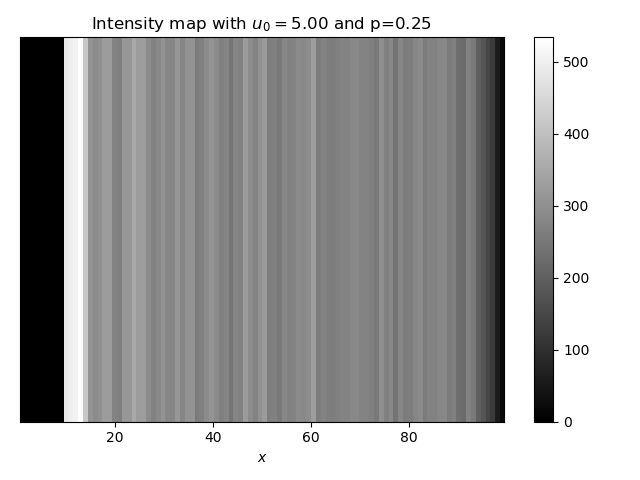
\includegraphics[scale=0.5]{fig3.png}  % Mention the image name within the curly braces. Image should be in the same folder as the tex file. 

   	\label{fig:sample}
   \end{figure} 
   
   
  \newpage
 \section{Table of count vs xpos}
 \begin{verbatim}
 +------+-------+
| xpos | count |
+------+-------+
| 0.5  |  0.0  |
| 1.5  |  0.0  |
| 2.5  |  0.0  |
| 3.5  |  0.0  |
| 4.5  |  0.0  |
| 5.5  |  0.0  |
| 6.5  |  0.0  |
| 7.5  |  0.0  |
| 8.5  |  0.0  |
| 9.5  | 487.0 |
| 10.5 | 499.0 |
| 11.5 | 506.0 |
| 12.5 | 534.0 |
| 13.5 | 416.0 |
| 14.5 | 309.0 |
| 15.5 | 294.0 |
| 16.5 | 302.0 |
| 17.5 | 327.0 |
| 18.5 | 326.0 |
| 19.5 | 277.0 |
| 20.5 | 265.0 |
| 21.5 | 317.0 |
| 22.5 | 315.0 |
| 23.5 | 353.0 |
| 24.5 | 326.0 |
| 25.5 | 328.0 |
| 26.5 | 293.0 |
| 27.5 | 272.0 |
| 28.5 | 287.0 |
| 29.5 | 309.0 |
| 30.5 | 283.0 |
| 31.5 | 280.0 |
| 32.5 | 317.0 |
| 33.5 | 280.0 |
| 34.5 | 310.0 |
| 35.5 | 310.0 |
| 36.5 | 257.0 |
| 37.5 | 268.0 |
| 38.5 | 293.0 |
| 39.5 | 307.0 |
| 40.5 | 292.0 |
| 41.5 | 269.0 |
| 42.5 | 279.0 |
| 43.5 | 246.0 |
| 44.5 | 278.0 |
| 45.5 | 272.0 |
| 46.5 | 325.0 |
| 47.5 | 292.0 |
| 48.5 | 277.0 |
| 49.5 | 304.0 |
| 50.5 | 325.0 |
| 51.5 | 263.0 |
| 52.5 | 267.0 |
| 53.5 | 255.0 |
| 54.5 | 283.0 |
| 55.5 | 271.0 |
| 56.5 | 276.0 |
| 57.5 | 291.0 |
| 58.5 | 286.0 |
| 59.5 | 293.0 |
| 60.5 | 328.0 |
| 61.5 | 262.0 |
| 62.5 | 273.0 |
| 63.5 | 264.0 |
| 64.5 | 261.0 |
| 65.5 | 269.0 |
| 66.5 | 274.0 |
| 67.5 | 272.0 |
| 68.5 | 284.0 |
| 69.5 | 284.0 |
| 70.5 | 277.0 |
| 71.5 | 276.0 |
| 72.5 | 269.0 |
| 73.5 | 255.0 |
| 74.5 | 300.0 |
| 75.5 | 269.0 |
| 76.5 | 285.0 |
| 77.5 | 244.0 |
| 78.5 | 283.0 |
| 79.5 | 260.0 |
| 80.5 | 262.0 |
| 81.5 | 280.0 |
| 82.5 | 292.0 |
| 83.5 | 260.0 |
| 84.5 | 273.0 |
| 85.5 | 273.0 |
| 86.5 | 283.0 |
| 87.5 | 284.0 |
| 88.5 | 258.0 |
| 89.5 | 269.0 |
| 90.5 | 232.0 |
| 91.5 | 224.0 |
| 92.5 | 276.0 |
| 93.5 | 255.0 |
| 94.5 | 202.0 |
| 95.5 | 178.0 |
| 96.5 | 148.0 |
| 97.5 | 123.0 |
| 98.5 |  59.0 |
| 99.5 |  22.0 |
+------+-------+

 \end{verbatim}
 \section{Conclusion}
 In the intensity vs x graph, the intensity reaches a maximum at around x = 15 and stays like that for around 5 bins and then decreases. This is because of the fact that the electron comes to rest after collision. Thus it has to gain energy from zero to be able to excite the atom for emmission of light. In the electron phase space graph, we can see from the graph the allowed velocities at a particular x. Thus we can say that the velocities are quantized. The number of electrons vs x graph shows the number of electrons which got excited at that value of x.
\end{document}



 